\section{System Development}

\subsection{UML Diagrams}

Some of the UML diagrams that we made for this system are given below.

\subsubsection{Use Case Diagram}

A use case diagram of our system is given in Figure \ref{fig:use-case}.

\begin{figure}[h]\centering
  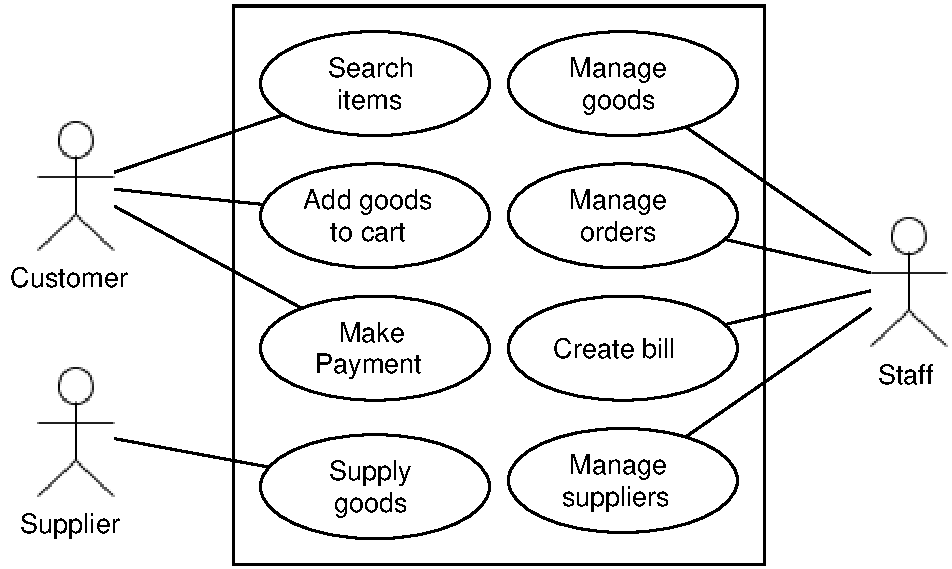
\includegraphics[width=4in]{fig/use-case}
  \caption{Use case diagram}\label{fig:use-case}
\end{figure}

\subsubsection{Class Diagram}

A Class Diagram in Unified Modeling Language (UML) is a type of static
structure diagram that describes the structure of a system by showing the
system's classes, their attributes, operations (or methods), and relationship
among objects. This diagram is considered as main building block of
object-oriented modelling. The classes in a class diagram represent both the
main element, interactions in the application,  and the classes to be
programmed. Each class comprises of three compartment, top compartment contains
name of class, middle compartment consist of attributes of the class and bottom
compartment contains methods that class can execute. Class diagram for DSMS is
shown below. The class diagram consist of instance level relationships.
Association represents a family of links and consist of role name,
multiplicity, navigational direction, visibility and other properties. Ex.
between product and supplier, the multiplicity is in a way that one supplier
can provide one or more product. The direction is from supplier to product and
role name is ``supplies'' indicating the statement ``Supplier provides one or
more product''. Similar is for other classes as well. Aggregation is ``has a''
association relationship. It represent that life of one class is dependent on
other. Ex. Bill\_detail is composite aggregate part (more strict) of Bill.
Generlization is shown in between Staff and other managers in diagram below.
what it signifies is that one of the two related class is considered to be
specialized form of the other. Here Staff is more general and *\_Manager is
specialized class. Other details are self explanatory and sufficient.



\begin{figure}[h]\centering
  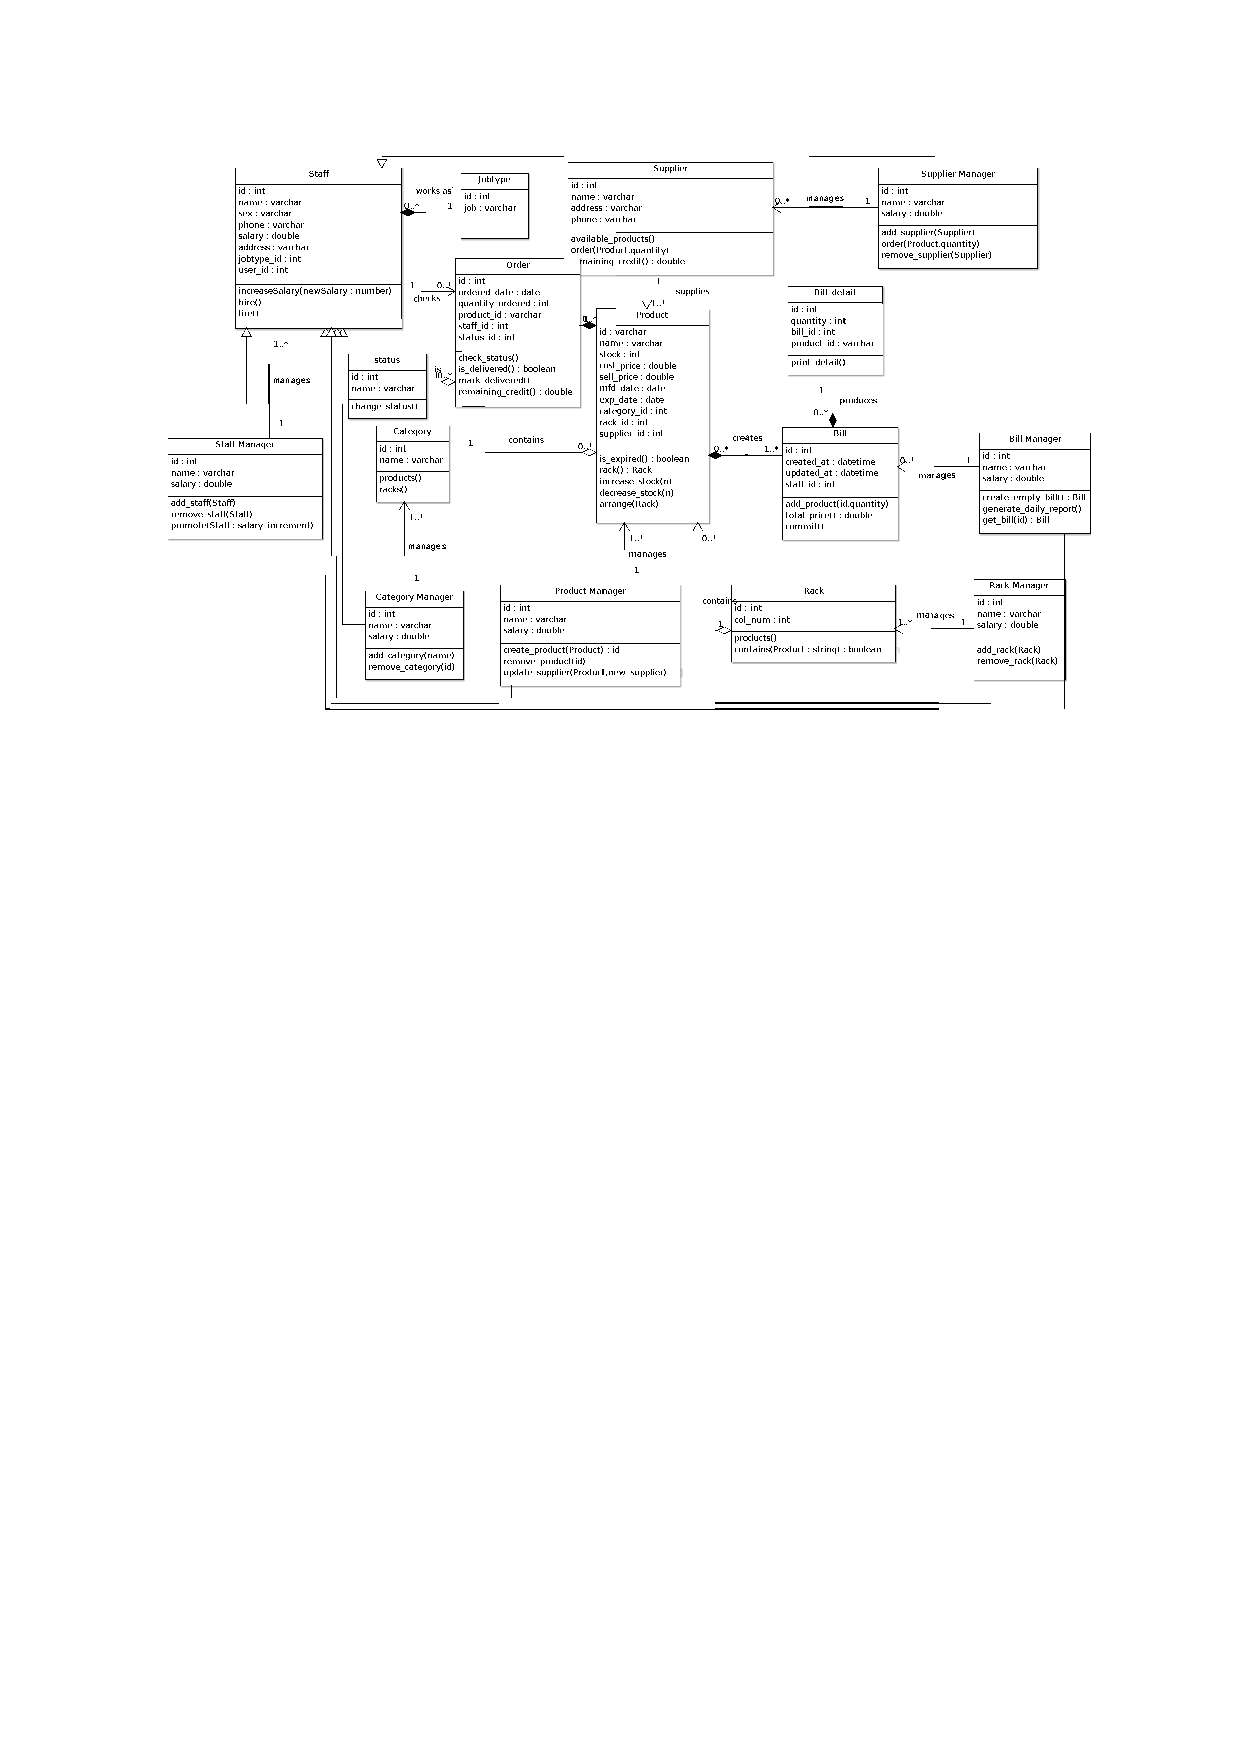
\includegraphics[width=\textwidth]{fig/class}
  \caption{Class diagram}\label{fig:class}
\end{figure}


\subsubsection{Sequence Diagram}

This diagram describes sequence of steps that may commonly occur in the
department store. We have five objects namely Department Store, Product,
Supplier, Customer, and Bill. Department Store checks for product status for
each product i.e. quantity (available stock), quality (exp date, condition
during storage), cost and updates the current status. Accordingly, it orders
goods/products from various suppliers and arrange them in store, Customers
come, search for product and buy required product. They find cost for each
product in label sticked to each product. A bill is made per transaction and
product is handed to customers after bill clearance. The activities like
searching product and buying product may happen several times (shown in diagram
explicitly as a loop). After the transaction is complete, store updates product
status and now has current status of the products.

Sequence diagram is an interaction diagram that shows how objects operate with
one another and in what order. It shows object interaction in time sequence.
The diagram shown is arranged in a way so that horizontal axis represent object
interaction (message exchange between objects) and vertical axis represent time
axis (life line of object). Some objects (like Bill) is created after
triggering particular event (here it is buy product) and destroyed after their
job is completed. The DSMS sequence diagram consist of five objects namely
Department Store, Product, Supplier, Customer, and Bill. Department Store
checks for product status for each product i.e. quantity (available stock),
quality (exp date, condition during storage), cost and updates the current
status. Accordingly, it orders goods/products from various suppliers and
arrange them in store, Customers come, search for product and buy required
product. They find cost for each product in label sticked to each product. A
bill is made per transaction and product is handed to customers after bill
clearance. The activities like searching product and buying product may happen
several times (shown in diagram explicitly as a loop). After the transaction is
complete, store updates product status and now has current status of the
products.

\begin{figure}[h]\centering
  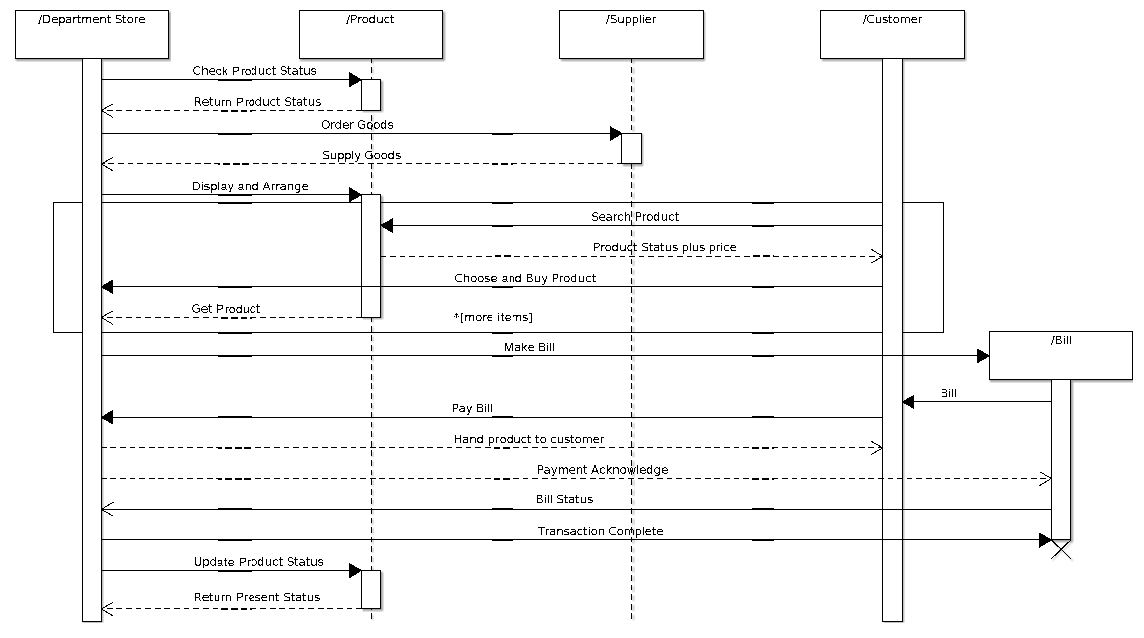
\includegraphics[width=\textwidth]{fig/sequence}
  \caption{Sequence diagram}\label{fig:sequence}
\end{figure}

\subsubsection{Activity Diagram}

Activity Diagram describes the dynamic aspects of the system. It diagram shows
user oriented view of system operation. We have made activity diagram using
swimlanes. A swim lane is a visual element that distinguishes job sharing and
responsibilities for sub-processes. In our system's activity diagram, we have
three swinlanes and we have separated job/responsibilities accordingly. Each
step is continuation of previous step. Decision is taken wherever necessary and
fork and join is used to divide or attach work flow. The objective of making
activity diagram is similar to objectives of other UML Diagrams. Only
difference is that it is used to show message flow between activities. Below is
the activity Diagram for DSMS. 

\begin{figure}[t]\centering
  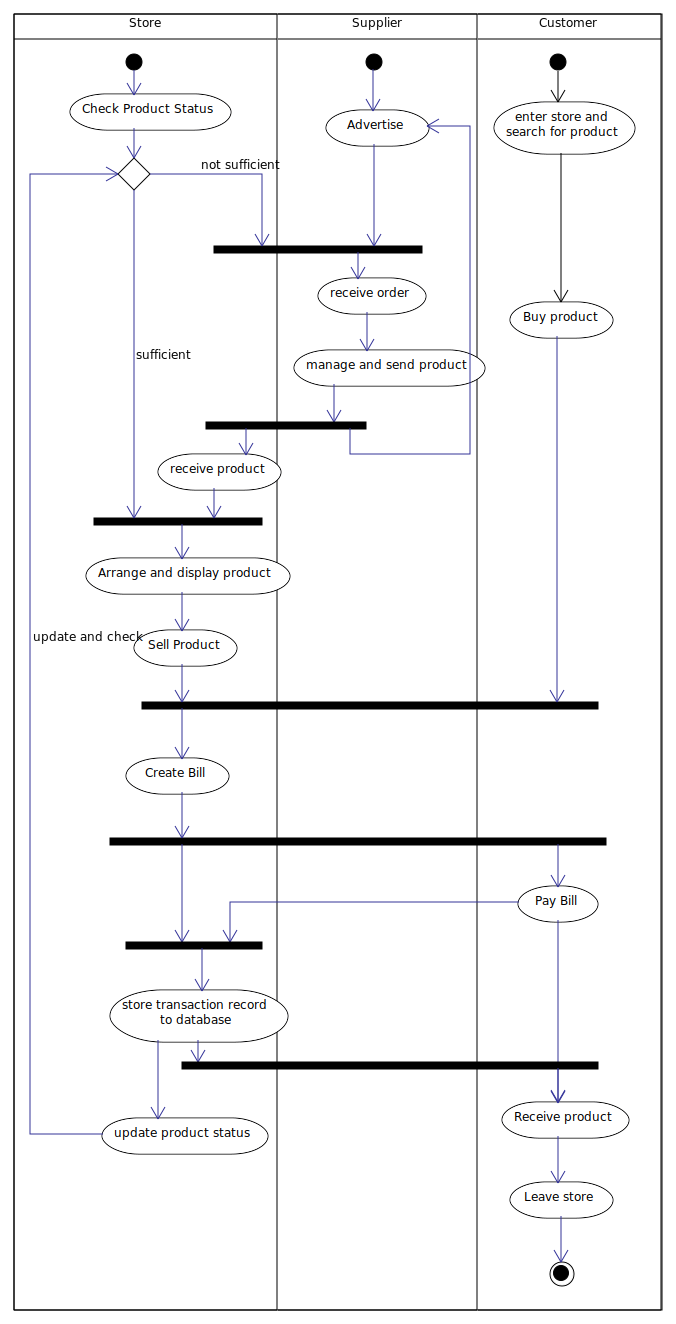
\includegraphics[height=\textheight-1cm]{fig/activity}
  \caption{Activity diagram}\label{fig:activity}
\end{figure}

\subsubsection{Collaboration Diagram}

Sequence diagram and collaboration diagram are very much similar to each other
that deals with instances and not classes. Collaboration (also called
communication) Diagram models the interaction between objects or parts in terms
of sequenced messages. This diagram is the combination of information taken
from Class, Sequence and Use Case Diagram describing both the static and
dynamic aspect of the system. Sequence diagram and collaboration diagram are
very much similar to each other that deals with instances and not classes and
it is easier to visualize the system from this diagram. Collaboration diagram
shows sequence of steps needed for operation of system in graph-like structure.
Sequence of step is explicitly written before each operation association
between instances. Collaboration Diagram for DSMS is shown below with five
instances and sequence of message exchange is shown explicitly by a number
before each message. Collaboration diagram shows interaction between element in
sequence but irrespective of time.

\begin{figure}[h]\centering
  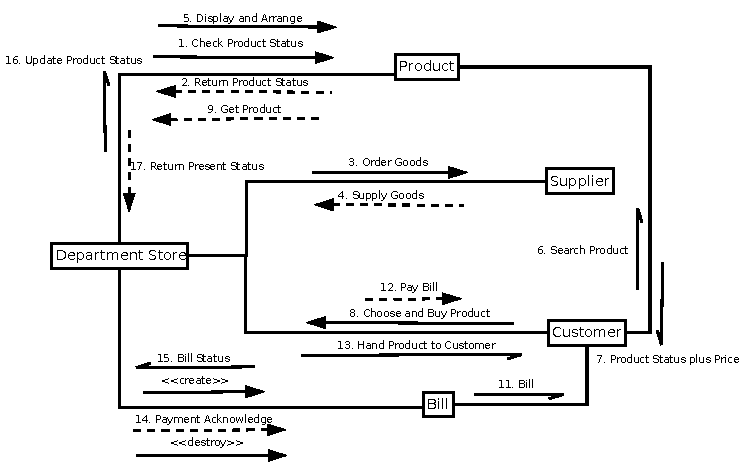
\includegraphics[width=\textwidth]{fig/collaboration}
  \caption{Collaboration diagram}\label{fig:collaboration}
\end{figure}

\subsubsection{State Chart Diagram}

State Chart Diagram describes a state machine. It models dynamic nature of a
system and defines different states of an object changed by events that occur
as the system runs. In the statie chart diagram of DSMS, events (may be
internal or external) is shown above each transition. Next state of the system
is determined by transition event and previous state. For ex. in ``Arrange
Product'' state, if event ``display'' is triggered, then it goes to ``Display
Product'' event and if ``sell'' event is triggered, it goes to ``Sell Product''
state. The state chart diagram for DSMS is shown below.

These diagrams depict the way in which objects evolve during their life in the
system. The elements of state chart diagram are:
\begin{description}
  \item[States] representing a stable condition of the object which persists
    for a significant time
  \item[Transitions] depicting possible paths from one state to another.
  \item[Events] these may be external events originating from actors, or
    internal events performed by other objects in the system.
  \item[Actions] processing carried out as part of a transition in state
  \item[Conditions] conditions governing the occurrence of a transition.
\end{description}

\begin{figure}[h]\centering
  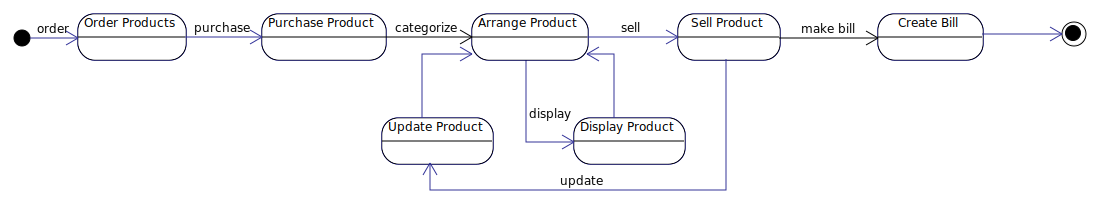
\includegraphics[width=\textwidth+1cm]{fig/state-chart}
  \caption{State chart diagram}\label{fig:state-chart}
\end{figure}


\subsection{Data Flow Diagrams}

Data flow diagram is used to show the flow of data from external entities into
the system. It is used to represent the physical and logical area of an
information system. The data flow diagrams are pictorial or graphical
representation of the Departmental Store Management System is shown below. The
data flow diagram covers all the processes and data storage area, which takes
place during any transaction in the system. Level 0 DFD is created after
identifying the logical subsystems that may exist in our system. The identified
subsystems are Customer Section, Supplier Section, Account Section and Central
Database. Only two external entities, namely Customer and Supplier take part in
DSMS. Logical Data Flow between customer and system include product search,
product info, product buy. Physical Data Flow includes Transaction receipt and
purchased goods/products. Similarly, supplier takes order from system (logical
data) and provide goods/product (physical data) to the system. Transaction
estimate bill and payment vouchers can also be considered as physical data
flow.

Level 1 DFD decomposes the processes in Level 0  DFD and identifies data
stores. There are separate DFD for Customer Section and Supplier Section. 

Customer Section is further divided into Counter (assist desk for customer),
Account (handles financial transaction between customer and system) and
database (data store for this section). Counter is only subsystem that
interacts with customer directly as well as other subsystem of the section.
Data Flow in this level is same as Level 0 data flow.

Similarly Supplier Section comprises of Administrator section, Account Section,
and Database. Administrator is responsible to make orders as per product
availability in stock and market rate. Supplier contacts this subsystem for all
dataflow mentioned in Level 0 DFD. Account section handles financial
tracsaction (payment---cash or check, old due, etc.) between supplier and system
and database is maintained to store all relevant information.

\begin{figure}[h]\centering
  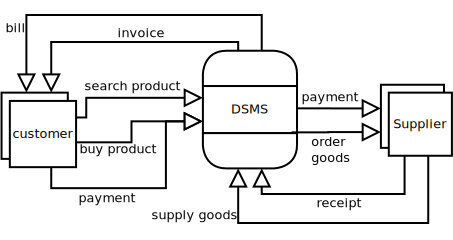
\includegraphics[width=4in]{fig/dfd-0}
  \caption{Level 0 (context) data flow diagram}\label{fig:dfd-0}
\end{figure}

\begin{figure}[h]\centering
  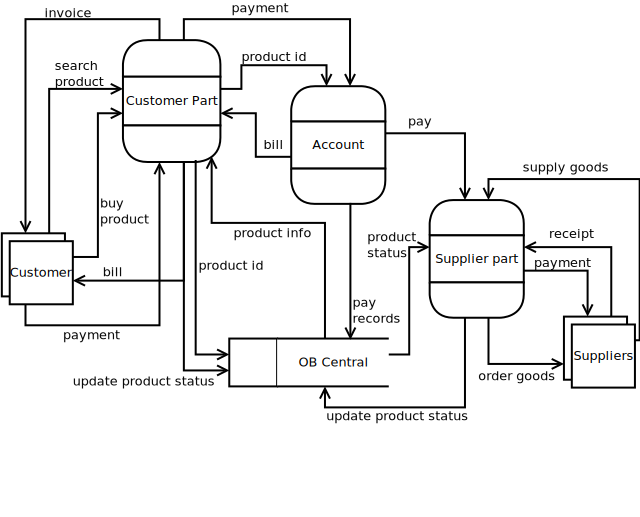
\includegraphics[width=5in]{fig/dfd-1}
  \caption{Level 1 data flow diagram}\label{fig:dfd-1}
\end{figure}

\begin{figure}[h]\centering
  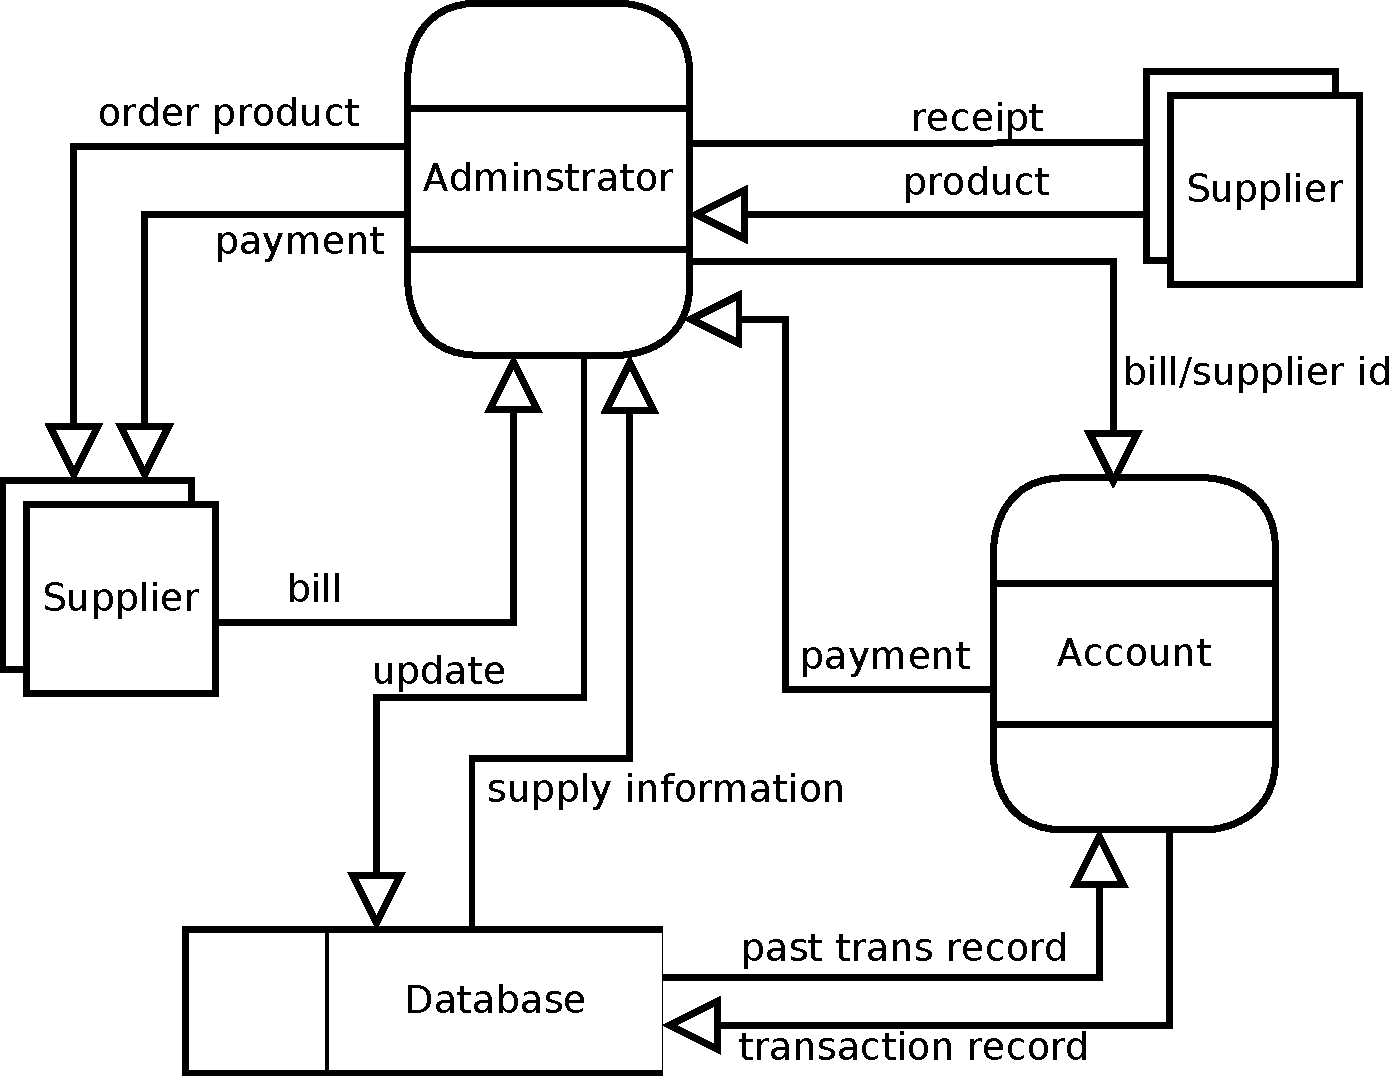
\includegraphics[width=4in]{fig/dfd-2}
  \caption{Level 2 data flow diagram}\label{fig:dfd-2}
\end{figure}

\begin{figure}[h]\centering
  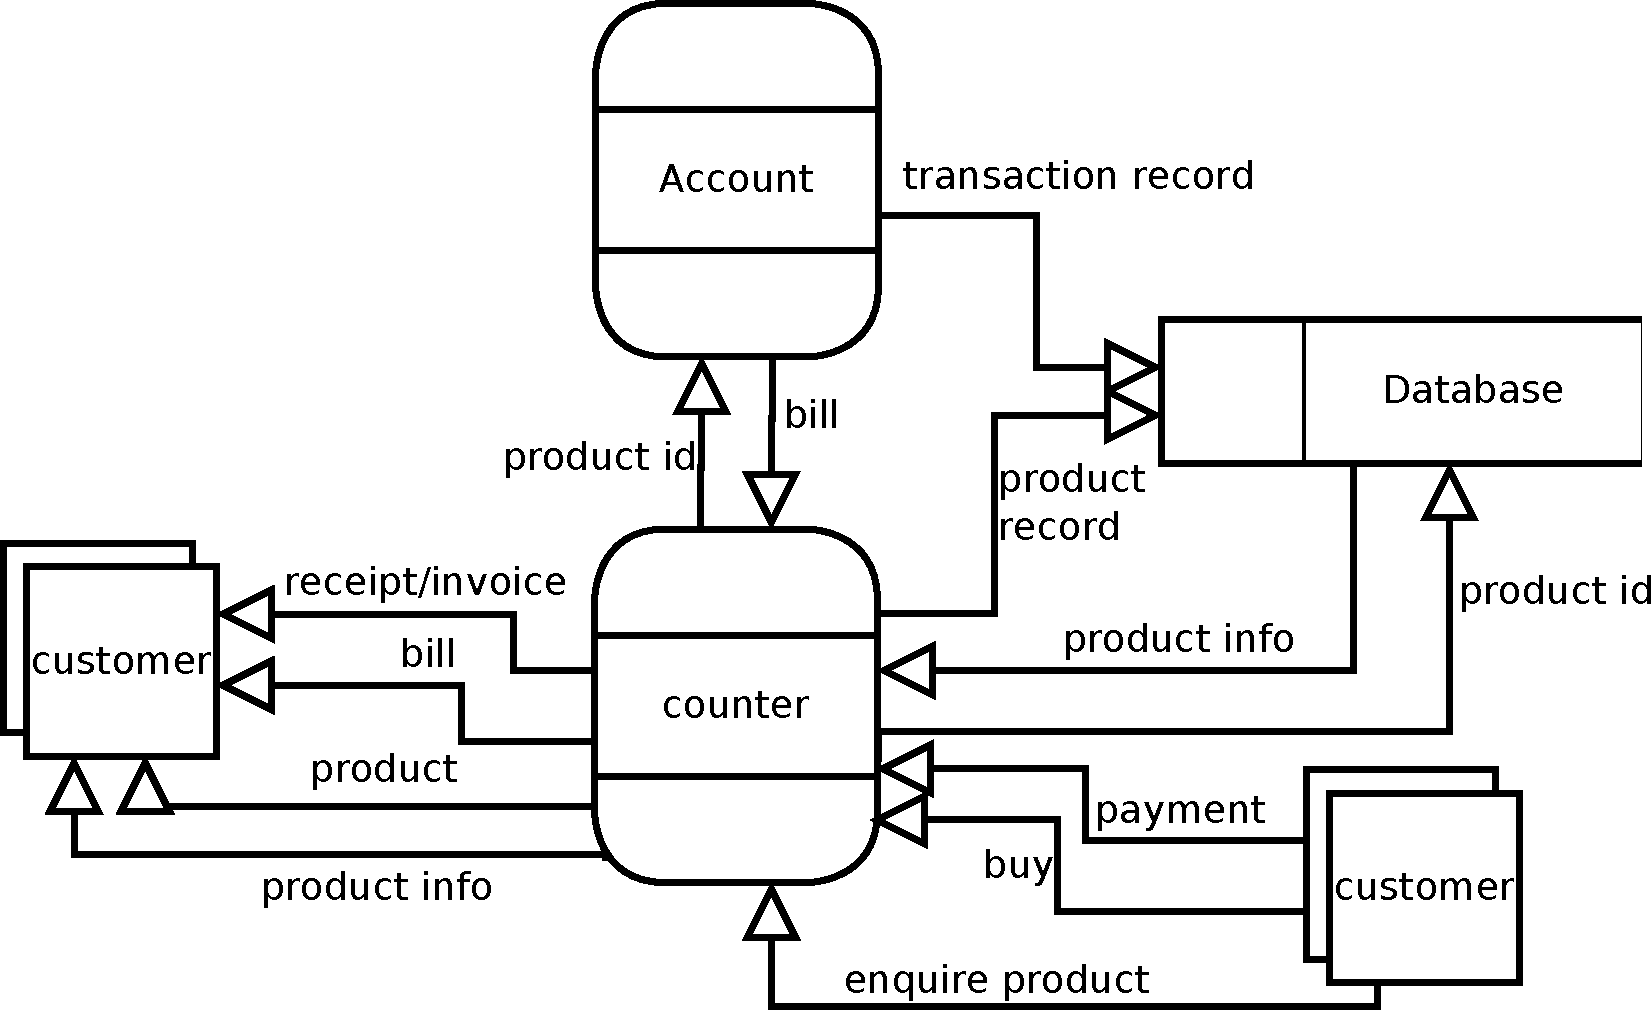
\includegraphics[width=5in]{fig/dfd-2-customer}
  \caption{Level 2 data flow diagram (customer)}\label{fig:dfd-2-customer}
\end{figure}

\subsection{Entity Relationship Diagrams}

An Entity-Relationship (ER) model describes inter-related things of interest in
a aspecific domain of knowledge. In software development, ER model ha become an
abstract data model that defines a data/information structure that can be
implemented in a database, typically a relational database. In our database, we
have separate tables for product, product category, supplier, bill, staff
details, order and other bunch of stuffs. Each table has several attributes
that best describe the table. To get required information, say we need to print
details of all transaction of particular day, then we need to access database
and more than one tables to retrieve data. We need certain relationship between
each tables in our database and a common attribute to map tuples of one table
to another. ER Diagram provides visual reference to complete database at one
glance. We can develop database looking at the ER Diagram and later use it as
reference for further improvement. The ER Diagram for DSMS is shown below.
Shown ER Diagram provides all tables, thier corresponding attributes, and
relationship among them.


\begin{figure}[h]\centering
  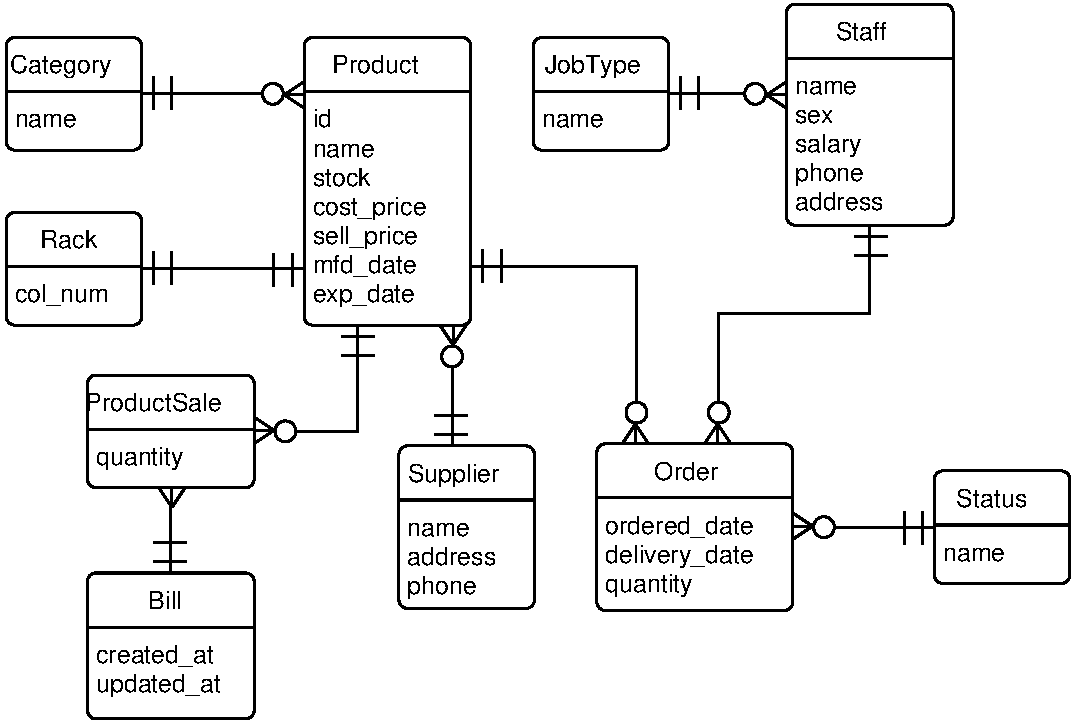
\includegraphics[width=\textwidth]{fig/erd}
  \caption{Entity relationship diagram}\label{fig:erd}
\end{figure}


\subsection{Project Schedule}

The project schedule is shown in the Gantt chart in Figure \ref{fig:gantt}.

\begin{figure}[h]\centering
  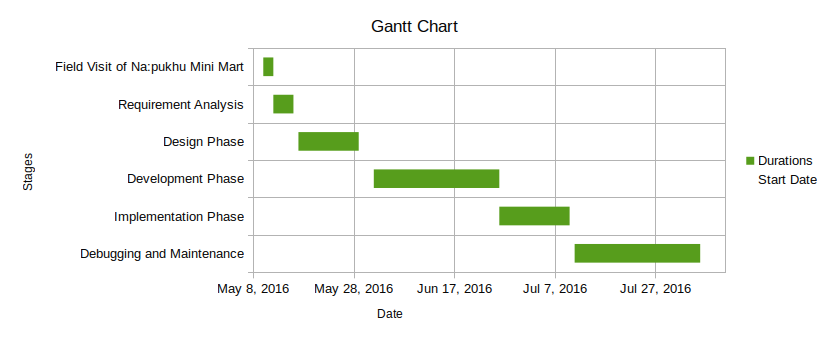
\includegraphics[width=\textwidth]{fig/gantt}
  \caption{Project Gantt chart}\label{fig:gantt}
\end{figure}
